\section{Open-Set Recognition}

Open-Set Recognition - метод распознавания с открытым набором параметров.
Порой может случиться так, что тестовый пример может быть визуально или метрически очень похожим на одну из категорий.
Наша задача - понять, когда эта кластеризация корректна, а когда мы делаем поспешные выводы.

\subsection{Основная идея}
Главной целью является попытка отличить похожие категории, которые были распознаны во время обучения, от новых, не идентифицированных. 
Другими словами, OSR специализируется на выявлении семантических сдвигов между категориями при обучении и тестировании.
Мотивацию можно представить как желание попытаться исключить ошибочное распознавание при близких параметрах, так как в реальном мире модели должны уметь не только различать объекты на существующих классах, но и идентифицировать случаи, когда сэмпл пришел из класса, который еще не встречался ранее.
Более инуитивное представление поможет получить картинка \ref{fig:anomalies-abstract}.

\begin{figure}[ht]
	\centering
	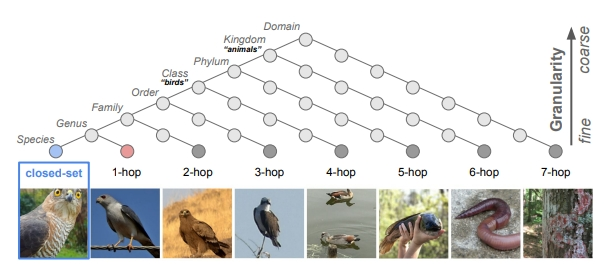
\includegraphics[width=0.8\linewidth]{chapters/anomalies/images/anomalies-abstract.jpg}
	\caption{Пример близких категорий из биологии}
	\label{fig:anomalies-abstract}
\end{figure}

На картинке мы видим, что чем дальше друг от друга виды животных на основе визуального восприятия, тем проще утверждать, что они относятся к разным классам и имеют более далеких предков.
Но чем ближе (пример - птицы), тем все труднее говорить о схожести видов, что может стать большой проблемой в силу некорректного отнесения животных к одному классу, роду или виду.
Иногда данная задача вызывает проблемы даже при попытке проделать ее самостоятельно, визуально.

\subsection{Постановка задачи}
Пусть у нас есть простанство объектов $X$, множество уже известных классов $Y = \{y_1, \dots, y_n\}$ и класс $u$ неизвестности, с которым мы как раз и должны научиться работать.

Модель в идеале должна сделать одно из двух следующих действий:
\begin{enumerate}
    \item Присвоить объекту $x \in X$ метку $y \in Y$, если объект принадлежит одному из известных классов.
    \item Присвоить метку $u$, если он не относится ни к одному из классов.
\end{enumerate}

\subsection{Методы}
\begin{enumerate}
    \item \textbf{На основе порога уверенности}
    
    Возьмем $S(x)$ за функцию, обозначающую отклик модели, он должен расти по мере роста $\mathcal{P}(y \in Y | x)$, где $y$ - предполагаемый класс объекта $x$. 
    Тогда:
    \begin{itemize} 
        \item Если $\max\limits_{y \in Y}{\mathcal{P}(y|x)}$ больше заранее определенного порога $\varepsilon$, то объект классифицируется моделью как принадлежащий $\hat{y} = \arg\max\limits_{y \in Y}{\mathcal{P}(y|x)}$.
        \item Если же меньше, то как неизвестный: $\hat{y} = u$
    \end{itemize}

    \item \textbf{На основе расстояний}
    
    Данный метод подходит если мы можем определить какую-либо метриуц на объектах.
    Метод основан на вычислении растояния от объекта до центров уже известных классов.
    
    Обозначим центры уже известных классов за $c_1, \dots, c_n$. 
    Обозначим за расстояние до центра $i$ за $d(x, c_i) = || x - c_i ||$. 
    Тогда:
    \begin{itemize}
        \item Если расстояние до ближайшего центра $cl(x) = \min\limits_{i}d(x, c_i)$ меньше заранее фиксированного порога $\varepsilon$, то объект классифицируется как принадлежащий $\hat{y} = \arg\min\limits_{i}d(x, c_i)$.
        \item Иначе же - как неизвестный: $y = u$.
    \end{itemize}
\end{enumerate}

По сути мы хотим минимизировать как количество ошибок классификации принадлежания одному из уже известных классов, так и отнесения к неизвестным объектам.
Стоит отметить, что при наличии явных выбросов или объектов, сильно отстояших от классов модель ложно отнесет их к неизвестным.

\subsection{Применение}
\begin{itemize}
    \item \textbf{Медицина}: распознавание и диагностика заболеваний, которые ранее могли быть еще не изучены или не встречаться
    \item \textbf{Биология}: пример с видами животных
    \item \textbf{Биометрия}: наверное самый наглядный пример, распознавание лица или отпечатка пальца человека. Мы должны сказать, является ли он известным или кто-то пытается взломать наш телефон
\end{itemize}

\subsection{Задачи}
Попробуйте ответить на следующие вопросы:

\problem Рассмотрим, как размер обучающей выборки для $n$ классов влияет на результат работы модели Open-Set Recognition. 
Формализуйте, как увеличение числа объектов в обучающей выборке может повлиять на вероятность ложных срабатываний и пропусков для неизвестных объектов.
\solution При небольшом размере обучающей выборки у модели не будет достаточной информации для точного определения границ между классами, что может привести к более высокому числу как ложных классификаций, так и ложных отнесений к неизвестному классу в силу отсутствия у нее возможности корректно научиться определять границы.

\problem Предложите метрику или способ обучения, которые вы бы использовали для оценки точности модели.
\solution С ходу понятно, как определять, что модель дала верный или не верный результат по уже известному классу. 
Но основная проблема состоит в том, чтобы оценить ее работу на объектах из неизвестного класса.
Давайте уберем из набора данных, используемого для тренировки часть, связанную с какими-либо известными классами, близкими к другим и будем валидировать способность нашей модели выделять неизвестные классы на ней.
Для оценки качества модели мы сможем применить метрику точности, равную отношению количества верных предсказаний в обоих случаях к общему количеству объектов:
$$Accuracy = \frac{TP + TR}{TP + TR + FP + FR},$$
где:
\begin{itemize}
    \item $TP$ - количество верных классификаций к одному из известных
    \item $TR$ - количество верных отнесений к неизвестному классу
    \item $FP$ - количество ошибочных кассификаций объекта как известного
    \item $FR$ - количество ошибочных отнесений объекта к неизвестным
\end{itemize}

\problem Предложите алгоритм, который можно было бы легко применить к задаче Open-Set Recognition.
\solution Давайте модифицируем логистическую регрессию. Для каждого класса $y_i$ она генерирует вероятность $\mathcal{P}(y_i|x)$, вычисляемую через сигмоидальную функцию.
Затем применим метод, основанный на пороге уверенности.

\section{Теория робастного (помехоустойчивого) обучения}
Традиционные методы обучения основываются на
том, что тренировочная выборка хорошо препроцессирована и не содержит шумов,
выбросов и недостающих значений. В реальных условиях хорошо структурировать
выборку не всегда возможно. В таких случаях на помощь могут прийти методы
робастного обучения.

Робастное обучение - это подход, фокусирующийся на построении моделей,
сохраняющих точность на неидеальных данных. Такая устойчивость обеспечивается
адаптивным подходам к входным данным. Методы обастного обучение частно
используют альтернативные функции потерь, алгоритмов, адаптирующихся к
структурам данных и/или детектирование и соответсвующую обработку аномалий.

\subsection{Схема итерационного взвешивания (IRS)}
IRS (Iterative Reweighting Scheme) - это один из
методов робасного обучения, заключающийся в обновлении весов объектов на каждом
шаге. Это позволяет уменьшить влияние аномальных данных. Вместо традиционных
функций потерь (таких как среднеквадратичная ошибка) в итерационной схеме
используются взвешенные функции потерь. IRS работает по следующему алгоритму:

\begin{enumerate}
  \item Инициализация весов
    Начинаем с иницаиализации весов:
    \[w_i^{(0)} = \frac{1}{l}, \forall i = 1, ..., l\]
  \item Обновление модели
    \[\alpha := arg min_{\alpha} \sum_{i=1}^l w_i L_i\left(\alpha\right) + \tau R\left(\alpha\right)\]

    \[w_i = norm_i\left( \mu^{'}\left( L_i(\alpha) \right) \right), i = 1, ..., l\]

    \[norm_i(v_i) = \frac{v_i}{\sum_j v_j}\]
  \item Повторяем обновление модели пока веса не стабилизируются или пока не
    будет достигнуто заданное число шагов
\end{enumerate}

\subsection{Задачи}
\subsubsection{Задача 1}
Предположим, что вы применили итеративную схему перевзвешивания на наборе
данных, содержащем выбросы. Вы применяете схему итеративного взвешивания.
По каким параметрам вы поймёте, чтоалгоритм сошёлся?
\textit{Ответ}: Веса изменяются не сильно, функция потерь перестала существенно
изменяться.
\subsubsection{Задача 2}
Предположим, что вы применили схему итерационного перевзвешивания к набору
данных и получили следующие веса на трех итерациях:
\[ w(1) = [0.40, 0.30, 0.20, 0.10] \]
\[ w(2) = [0.45, 0.25, 0.20 ,0.10] \]
\[ w(3) = [0.43, 0.26, 0.20, 0.10] \]

Считая критерием сходимости изменение весов и порог \(\epsilon = 0.01\),
скажите, сошёлся ли алгоритм/
\textit{Ответ}:
\[ \Delta w^{1\rightarrow2} = max\left( \abs{0.4-0.45}, \abs{0.3 - 0.25}, \abs{0.2-0.2}, \abs{0.1-0.1}  \right) = 0.05 \]
\[ \Delta w^{2\rightarrow3} = max\left( \abs{0.43-0.45}, \abs{0.26 - 0.25}, \abs{0.2-0.2}, \abs{0.1-0.1}  \right) = 0.02 \]
Т.к. обе дельты больше \(\epsilon\), то алгоритм не сошёлся.

\subsubsection{Задача 3}
Хоошо ли работают алгоритмы итеративного перевзвешивания на данных с высокой
мультиколлинеарностью?
\textit{Ответ}: Работает плохо, т.к. в алгоритме перевзвешивания веса объектов
обновляются независимо, а значит, изменение веса одного объекта не влияет на
вес второго. В случае высокой зависимости между данными этот подход не может
быть применён, т.к. они требуют согласованного изменения весов кореллирующих
объектов.

\section{PU-Learning}

PU-Learning (Positive-Unlabeled Learning) — это метод машинного обучения, в котором имеются только положительные примеры и неразмеченные данные. Такой подход применим в случаях, когда отсутствуют отрицательные метки, а задача состоит в выявлении скрытых закономерностей среди неопределенных данных.

\subsection{Основная идея}

Цель PU-Learning — построить модель, которая различает положительные и отрицательные примеры, несмотря на то, что в обучающем наборе отсутствуют явные отрицательные метки. Примеры задач PU-Learning включают:

\begin{itemize}
    \item обнаружение мошеннических транзакций;
    \item рекомендательные системы и персонализация рекламы;
    \item автоматическое пополнение базы знаний фактами.
\end{itemize}

Для решения задачи PU-Learning неразмеченные объекты трактуются как негативные с весом \( C_- \ll C_+ \), где \( C_+ \) — вес для положительных примеров. Проблема сводится к минимизации следующей функции потерь:

\[
\sum_{i=1}^k \frac{C_+}{k} \mathcal{L}(a(x_i, w), +1) + \sum_{i=k+1}^\ell \frac{C_-}{\ell - k} \mathcal{L}(a(x_i, w), -1) + \tau R(w) \to \min_w,
\]

где \( a(x_i, w) \) — функция классификации, \( \mathcal{L} \) — функция потерь, \( R(w) \) — регуляризация, \( \tau \) — коэффициент регуляризации.

\subsection{Постановка задачи}

Пусть дана выборка \( X = \{x_1, x_2, \dots, x_\ell\} \), где:
\begin{itemize}
    \item \( P \subset X \) — положительные примеры с меткой \( y = +1 \),
    \item \( U = X \setminus P \) — неразмеченные данные.
\end{itemize}

Задача заключается в построении модели \( a(x, w) \), которая будет классифицировать объекты \( x \in U \) на положительные и отрицательные классы, минимизируя ошибку классификации при отсутствии явных негативных примеров.

\subsection{Методы}

\textbf{Biased SVM.} Один из наиболее успешных методов PU-Learning — это Biased Support Vector Machine (Biased SVM). Основная идея заключается в следующем:
\begin{itemize}
    \item Положительные примеры из \( P \) используются как основной класс.
    \item Неразмеченные объекты из \( U \) рассматриваются как негативные, но с меньшим весом \( C_- \).
\end{itemize}

Формально задача оптимизации выглядит как:

\[
\min_w \sum_{i=1}^k \frac{C_+}{k} \mathcal{L}(a(x_i, w), +1) + \sum_{i=k+1}^\ell \frac{C_-}{\ell - k} \mathcal{L}(a(x_i, w), -1) + \tau R(w),
\]

где веса \( C_+ \) и \( C_- \) регулируют вклад положительных и неразмеченных объектов в общую функцию потерь.

\textbf{Метод на основе вероятностной модели.} В альтернативном подходе используется вероятность принадлежности объекта \( x \) положительному классу. Предполагается, что неразмеченные данные представляют смесь положительных и отрицательных примеров, и задача сводится к оценке вероятности \( p(y = +1 | x) \).

\subsection{Задачи}

\problem Постройте функцию потерь для задачи PU-Learning, если известно, что положительные примеры имеют больший вес \( C_+ \), а неразмеченные данные трактуются как негативные с весом \( C_- \ll C_+ \).

\solution Функция потерь будет иметь следующий вид:
\[
\sum_{i=1}^k \frac{C_+}{k} \mathcal{L}(a(x_i, w), +1) + \sum_{i=k+1}^\ell \frac{C_-}{\ell - k} \mathcal{L}(a(x_i, w), -1) + \tau R(w).
\]
Здесь первая сумма учитывает положительные примеры, а вторая — неразмеченные объекты с меньшим весом \( C_- \).

\problem Какие трудности могут возникнуть при использовании метода Biased SVM для PU-Learning?

\solution Основные трудности включают:
\begin{itemize}
    \item некорректное назначение неразмеченных данных как отрицательных, что может привести к смещению модели;
    \item выбор оптимального соотношения весов \( C_+ \) и \( C_- \), что требует дополнительной настройки;
    \item необходимость регуляризации для избежания переобучения модели на положительных примерах.
\end{itemize}

\problem Как можно оценить качество модели PU-Learning при отсутствии явных отрицательных примеров?

\solution Одним из подходов является использование метрики AUC (Area Under the Curve), которая позволяет оценить способность модели различать положительные и отрицательные примеры, даже если отрицательные метки не представлены явно.

\section{One-Class Classification}

One-Class Classification (OCC) — это метод машинного обучения, предназначенный для выявления аномалий или отклонений, когда в обучающих данных представлены только объекты одного класса (нормальные данные). Этот подход полезен в ситуациях, когда сбор данных об аномалиях затруднен или невозможен.

\subsection{Основная идея}

Главная цель One-Class Classification заключается в построении модели, которая будет определять границу между нормальными и аномальными объектами. При этом аномальные объекты считаются редкими или сильно отличающимися от нормальных данных. Задача заключается в том, чтобы минимизировать количество ложных положительных и отрицательных решений при отсутствии информации о "аномальном" классе.

Примеры применения One-Class Classification включают:
\begin{itemize}
    \item обнаружение дефектов на производственных линиях;
    \item выявление несанкционированных вторжений в системы безопасности;
    \item диагностика сбоев в инженерных системах.
\end{itemize}

Одним из наиболее популярных методов One-Class Classification является \textbf{One-Class SVM}, который строит гиперплоскость, отделяющую нормальные объекты от остального пространства с минимизацией объема области, содержащей нормальные данные.

\subsection{Постановка задачи}

Пусть дана выборка \( X = \{x_1, x_2, \dots, x_n\} \), состоящая только из нормальных объектов. Необходимо построить модель \( f(x) \), которая будет удовлетворять следующим условиям:
\begin{itemize}
    \item Для нормальных объектов \( x \in X \): \( f(x) = 1 \).
    \item Для аномальных объектов \( x \notin X \): \( f(x) = -1 \).
\end{itemize}

Таким образом, задача сводится к построению разделяющей поверхности, которая включает максимальное количество нормальных данных и минимизирует область, отведенную для аномалий.

\subsection{Методы}

\textbf{One-Class SVM.} В основе метода One-Class SVM лежит построение гиперплоскости, которая максимально отделяет нормальные объекты от остального пространства. Задача оптимизации для One-Class SVM выглядит следующим образом:

\[
\min_{\mathbf{w}, \xi, \rho} \frac{1}{2} \|\mathbf{w}\|^2 + \frac{1}{\nu n} \sum_{i=1}^n \xi_i - \rho
\]
при ограничениях:
\[
(\mathbf{w} \cdot \phi(x_i)) \geq \rho - \xi_i, \quad \xi_i \geq 0, \quad i = 1, \dots, n.
\]

Здесь:
\begin{itemize}
    \item \( \mathbf{w} \) — нормаль к гиперплоскости;
    \item \( \phi(x) \) — функция преобразования данных в пространство большей размерности;
    \item \( \xi_i \) — переменные, отвечающие за ошибки классификации;
    \item \( \rho \) — пороговое значение, определяющее границу разделения;
    \item \( \nu \) — параметр, контролирующий количество допустимых ошибок.
\end{itemize}

\textbf{Автоэнкодеры для OCC.} В нейросетевых подходах для One-Class Classification часто используются автоэнкодеры. Модель обучается на нормальных данных минимизировать ошибку восстановления. Аномальные объекты, которые значительно отличаются от нормальных, имеют высокую ошибку восстановления и таким образом выявляются как аномалии.

\subsection{Задачи}

\problem Как можно построить модель One-Class SVM для выявления аномалий, если обучающая выборка содержит только нормальные данные?

\solution Для построения модели One-Class SVM необходимо использовать нормальные данные для обучения гиперплоскости, которая отделяет их от остального пространства. Параметр \( \nu \) контролирует степень "доверия" модели к данным и позволяет регулировать количество допустимых ошибок при классификации.

\problem Как автоэнкодеры могут использоваться для задач One-Class Classification?

\solution Автоэнкодеры обучаются на нормальных данных восстанавливать их с минимальной ошибкой. При подаче на вход аномальных данных ошибка восстановления значительно увеличивается, так как модель не обучена работать с такими объектами. Таким образом, высокая ошибка восстановления используется в качестве критерия для выявления аномалий.

\problem Какие метрики можно использовать для оценки качества модели One-Class Classification, особенно в случае несбалансированных данных?

\solution В задачах One-Class Classification для оценки качества модели рекомендуется использовать метрику ROC AUC, которая позволяет оценить способность модели различать нормальные и аномальные объекты. Эта метрика не зависит от несбалансированности данных и поэтому подходит для задач с редкими аномалиями.




\section{Итерационное перевзвешивание для произвольной агрегирующей функции. Алгоритм IR-ERM.}

Существует проблема искажения значения функции потерь из-за выбросов. Идея такова: изменить веса у функций потерь на тренировочных данных, чтобы учитывать влияние выбросов, уменьшая влияние больших значений функций потерь. Методы IRS и IRLS помогают совершить задуманное, но являются недостаточно подходящими из-за ограничений на агрегирующую функцию. Для более устойчивых к выбросам функций, таких как медиана, они не подходят. Таким образом, требуется создать новый метод, позволяющий совершить перевзвешивание уже для произвольных агрегирующих функций.

\subsection{Алгоритм IR-ERM. Теория}

Сначала немного определений. Обобщённая задача минимизации эмпирического риска (ERM) выражается так:
$$Q(\alpha) = M(\mathscr{L}_1(\alpha), \mathscr{L}_2(\alpha), ... \mathscr{L}_N(\alpha)) + \tau R(\alpha) \xrightarrow{} \underset{\alpha}{min}$$

При этом $M$ является той самой агрегирующей функцией. Тогда при искомом значении $\alpha$
$$\nabla Q(\alpha) = \sum_{i=1}^N \frac{\delta M}{\delta \mathscr{L}_i}(\mathscr{L}_1(\alpha), \mathscr{L}_2(\alpha), ..., \mathscr{L}_N(\alpha)) \nabla \mathscr{L}_i(\alpha) + \tau \nabla R(\alpha) = 0$$

Исходя из минимизации влияния выбросов, веса должны быть как раз такими: $w_i = \frac{\delta M}{\delta \mathscr{L}_i}(\mathscr{L}_1(\alpha), \mathscr{L}_2(\alpha), ..., \mathscr{L}_N(\alpha)) \nabla \mathscr{L}_i(\alpha)$. Исходя из этого выстраивается идея итерационного алгоритма перевзвешивания:

Инициализируем $w_i = \frac{1}{N}, i = 1,...,N$

повторять
\begin{quote}
    $\alpha := arg \; \underset{\alpha}{min} \sum_{i=1}^N w_i \mathscr{L}_i(\alpha) + \tau R(\alpha)$\
    
    $w_i := \frac{\delta M}{\delta \mathscr{L}_i}(\mathscr{L}_1(\alpha), \mathscr{L}_2(\alpha), ..., \mathscr{L}_N(\alpha)) \nabla \mathscr{L}_i(\alpha)$
\end{quote}

пока веса $w_i$ не стабилизируются.

Сразу возникает вопрос: как в случае таких робастных оценок как нахождение медианы получить частную производную, ведь функция не является дифференцируемой? Найдём ответ и к этому.

Медиану можно выразить так: $M(z_1, ..., z_N) = arg \; \underset{u}{min} \sum_{i=1}^N |z_i - u|$. Сам по себе модуль не является дифференцируемой функцией, из-за чего непонятно, как получить производную, но это уже продвижение. И теперь его можно заменить на гладкую функцию, близкую к настоящему модулю. Как вариант, сглаженный модуль: $d_{\epsilon}(x) = \sqrt{\epsilon ^ 2 + x^ 2} - \epsilon \xrightarrow{} 0$, при $\epsilon \xrightarrow{} 0$.
Для $\gamma$ квантили уже подходит вариант со сглаженным несимметричным модулем:
\[
    d_{\gamma \epsilon}(x)= 
\begin{cases}
    2\gamma d_{\epsilon}(x),& x \geq 0\\
    2(1 - \gamma) d_{\epsilon}(x),& x < 0
\end{cases}
\]

Теперь, используя эту идею, запишем $M(z_1, ..., z_N) =  arg \underset{u}{min} \sum_{i=1}^N d(z_i - u)$, где $d$ как раз является такой гладкой функцией (пока не будем утверждать, что это модуль или что-то ещё такое). Поскольку значение $M$ ищется как точка минимума, запишем условие на производную: $\sum_{i=1}^N d'(z_i - M) = 0$, продифференцируем его по $z_k$ и найдём наконец $\frac{\delta M}{\delta z_k}$:
$$\sum_{i=1}^Nd''(z_i - M) \frac{\delta}{\delta z_k} (z_i - M) = 0$$
$$d''(z_k - M) = \frac{\delta M}{\delta z_k} \sum_{i=1}^Nd''(z_i - M)$$
$$\frac{\delta M}{\delta z_k} = \frac{d''(z_k - M)}{\frac{\delta M}{\delta z_k} \sum_{i=1}^Nd''(z_i - M)} = \underset{k}{norm} \; d''(z_k - M)$$
где $\underset{k}{norm}$ обозначает нормировку.

Теперь осталось научиться решать уравнение $u \equiv M$.

Для решения такой задачи $\sum_{i=1}^Nd'(z_i - M) = 0$ методом итераций можно представить $M = f(M)$.
$$\sum_{i=1}^N \frac{d'(z_i - M)}{(z_i - M)} (z_i - M) = 0$$
$$\sum_{i=1}^N \frac{d'(z_i - M)}{(z_i - M)} z_i = \sum_{i=1}^N \frac{d'(z_i - M)}{(z_i - M)} M$$
$$M = \frac{\sum_{i=1}^N z_i \phi(z_i - M)}{\sum_{i=1}^N M \phi(z_i - M)} = \sum_{i=1}^N z_i \; \underset{i}{norm} \; \phi(z_i - M), \quad \phi(x) = \frac{d'(x)}{x}$$

Таким образом, изначально инициализируется значение $M$, после, пока оно не сойдётся, к нему применяется данная функция $f$. Процесс $M_{t+1} = f(M_t)$ сходится, если $|f'(M)| < 1$ в окрестности неподвижной точки $M = f(M)$. Проверим это:

$$\left|\frac{\delta}{\delta M} \frac{\sum_{i=1}^N z_i \phi(z_i - M)}{\sum_{i=1}^N M \phi(z_i - M)}\right| < 1$$
$$\left|\frac{\sum_{i=1}^N (z_i - M) \phi'(z_i - M)}{\sum_{i=1}^N M \phi(z_i - M)}\right| < 1$$

Это условие уже нетрудно проверить для используемых $d$.

Обобщим всё вместе и получим полный алгоритм:

Инициализация $w_i = \frac{1}{N}, i = 1,...,N$

повторять
\begin{quote}
    $\alpha := arg \; \underset{\alpha}{min} \sum_{i=1}^N w_i \mathscr{L}_i(\alpha) + \tau R(\alpha)$\
    
    $z_i := \mathscr{L}_i(\alpha)$\
    
    инициализируем $M = \sum_{i=1}^N w_i z_i$\

    повторять\
    \begin{quote}
        $M = \sum_{i=1}^N z_i \; \underset{i}{norm} \; d''(z_k - M)$\
    \end{quote}
    
    пока M не сойдётся\
    
    $w_i := \underset{i}{norm} \; d''(z_k - M) \nabla \mathscr{L}_i(\alpha)$ \

\end{quote}

пока $w_i$ не стабилизируются

На входе алгоритма функции потерь $\mathscr{L}_i$, на выходе — оптимальные значения параметров модели и весов.

\subsection{Задачи}

\problem

Почему стоит вообще использовать алгоритмы итерационного взвешивания? Какие их преимущества над простым удалением выбросов? 

\begin{solution}
    При удалении выбросов мы теряем их влияние на результат вовсе, уменьшая тренировочную выборку, при этом, если они являются просто зашумленными данными, в целом давая правильные результаты, то лучше будет просто уменьшить их влияние, но оставить для более полной оценки. Кроме того, при нахождении весов мы получаем достаточно важную характеристику для данных — показатель шума, влияния на результат обучения.
\end{solution}

\problem

Есть датасет о посещаемости сети картинг-центров на протяжении десяти лет. Требуется обучить на этих данных модель для предсказаний, сколько посетителей ждать в определённый день. Доступны данные о погоде, о том, какой сейчас день недели, выходной или нет, какое время года. Также было бы неплохо промаркировать случаи с выбросами, когда в определённый день пришло заметно больше или меньше человек, чем должно быть. Что в данном случае предпочтительнее использовать, IRS или IR-ERM? Почему?


\begin{solution}

    С точки зрения данной задачи выгоднее использовать IR-ERM и вот почему. Посещаемость сильно зависит от непредсказуемых факторов, от праздников, от рекламы, от роста населения. Поэтому выбросов должно быть очень много, причём есть несколько сильно отличающихся от предсказанных результатов. Таким образом, ради избавления от сильно смещённой оценки, которая может получиться при использовании IRS, которая пасует при большом количестве выбросов, стоит использовать IR-ERM.

\end{solution}


\problem

Проверьте, что IR-ERM действительно работает, если как $M$ взять среднее арифметическое.

\begin{solution}
    В случае взятия $M$ как среднего арифметического, можно просто воспринимать, что $M(z_1,...,z_N) = arg \; \underset{u}{min} \sum_{i=1}^N (z_i - u)^2$. Тогда получается, что $d(x) = x^2$, для работы алгоритма требуется проверить итерационную сходимость функции $f$, что сработает, поскольку $\phi (x) = \frac{2x}{x} = 2, \phi'(x) = 0, f'(M) = \frac{\sum_{i=1}^N (z_i - M) \phi'(z_i - M)}{\sum_{i=1}^N M \phi(z_i - M)} = 0$,
    $|f'(M)| < 1$. Остальные рассуждения выполняются так или иначе, поэтому алгоритм сойдётся.
\end{solution}

\section*{Семейство робастных агрегирующих функций}
Агрегирование данных — важная задача в машинном обучении. Традиционные методы усреднения, такие как арифметическое среднее, оказываются неустойчивыми к выбросам, что приводит к некорректным результатам. Робастные агрегирующие функции решают эту проблему, обеспечивая устойчивость к аномальным значениям.

Рассмотрим вариационный ряд $z^{(1)} \leq ... \leq z^{(t)}$ значений $z_1, z_2, \dots, z_\ell$. Классические и робастные методы усреднения можно формализовать как задачу минимизации функции \textit{несходства} $d(z_i - u)$ по параметру $u$:
\begin{equation}
    M(z_1, \dots, z_\ell) = \arg \min_u \sum_{i=1}^\ell d(z_i - u).
\end{equation}
Здесь $M(z_1, \dots, z_\ell)$ — агрегирующая функция, а $d(r)$ — функция несходства, обладающая следующими свойствами:
\begin{itemize}
    \item $d(r) \geq 0, \; d(0) = 0$;
    \item строго выпуклая функция.
\end{itemize}

\section*{Примеры робастных агрегирующих функций}
\subsection*{1. Медиана}
Медиана определяется как значение, минимизирующее сумму модулей отклонений:
\begin{equation}
    M(z_1, \dots, z_\ell) = \arg \min_u \sum_{i=1}^\ell |z_i - u|.
\end{equation}
Она устойчива к выбросам, так как небольшое число аномальных значений не влияет на её положение.

\subsection*{2. $\gamma$-квантиль}
Обобщением медианы является $\gamma$-квантиль, которая учитывает весовую асимметрию:
\begin{equation}
    M(z_1, \dots, z_\ell) = \arg \min_u \sum_{i=1}^\ell |z_i - u| \cdot \begin{cases}
        \gamma, & z_i \geq u, \\
        1 - \gamma, & z_i < u.
    \end{cases}
\end{equation}

\subsection*{3. Цензурированное среднее}
Цензурированное среднее определяется как минимум между значением $z_i$ и некоторым порогом $z^{(m)}$:
\begin{equation}
    M(z_1, \dots, z_\ell) = \frac{1}{\ell} \sum_{i=1}^\ell \min(z_i, z^{(m)}).
\end{equation}
Цензурирование позволяет ограничить влияние аномальных значений.

\section*{Сглаженные функции несходства}
Проблема минимизации функций, таких как модуль $|z_i - u|$, заключается в их недифференцируемости в точке $r = 0$. Решением является использование \textit{сглаженных функций} несходства.

\subsection*{Сглаженный модуль}
Для приближения медианы используется сглаженный модуль $d_\varepsilon(r)$:
\begin{equation}
    d_\varepsilon(r) = \sqrt{\varepsilon^2 + r^2} - \varepsilon, \quad \varepsilon \to 0.
\end{equation}
Эта функция дифференцируема, а при $\varepsilon \to 0$ она стремится к $|r|$.

\subsection*{Сглаженный асимметричный модуль}
Для $\gamma$-квантиля используется сглаженная асимметричная функция:
\begin{equation}
    d_{\gamma\varepsilon}(r) = \begin{cases}
        2\gamma d_\varepsilon(r), & r \geq 0, \\
        2(1 - \gamma) d_\varepsilon(r), & r < 0.
    \end{cases}
\end{equation}

\subsection*{Cглаженное цензурированное среднее}
Цензурированное среднее можно аппроксимировать с помощью сглаженного модуля. Используя тождество:
\begin{equation}
    \min(z_i, u) = \frac{1}{2}(z_i + u) - \frac{1}{2}|z_i - u|,
\end{equation}
получаем сглаженную версию:
\begin{equation}
    M(z_1, \dots, z_\ell) = \frac{1}{2\ell} \sum_{i=1}^\ell \left[ z_i + z_{\gamma\varepsilon} - d_\varepsilon(z_i - z_{\gamma\varepsilon}) \right],
\end{equation}
где $z_{\gamma\varepsilon}$ определяется как решение задачи минимизации:
\begin{equation}
    z_{\gamma\varepsilon} = \arg \min_u \sum_{i=1}^\ell d_{\gamma\varepsilon}(z_i - u).
\end{equation}

\section*{Задачи}
Докажите свойства агрегирующей функции
\subsection*{1. Монотонность}
{Если } z_i \leq z_i' , \text{ то } M(z_1, \dots, z_l) \leq M(z_1', \dots, z_l').
\subsection*{2. Симметричность}
M(z_1, \dots, z_l) = M(z_{\pi(1)}, \dots, z_{\pi(1)}) \text{ для } \forall \pi
\subsection*{3. Среднее по Коши}
\min_i{{z_i}} \leq M(z_1, \dots, z_t) \leq max_i{{z_i}}
